\section{Methods}


\begin{frame}{Fiber Construction}{Informal Definition: Beyond the scope of this presentation}

\small
\begin{itemize}
    \item A construction that expresses the semantics of \emph{remote attribute grammars} in \emph{classical terms}
    \item Objects implicitly carry separate values for the fields is like a \alert{rope} which can be separated into the individual fibers
    \item This yields a corrupt attribute grammar with an infinite number of attributes
    \item \emph{fiber approximation} fixes that (which then may include cycles ...)
\end{itemize}

\begin{center}
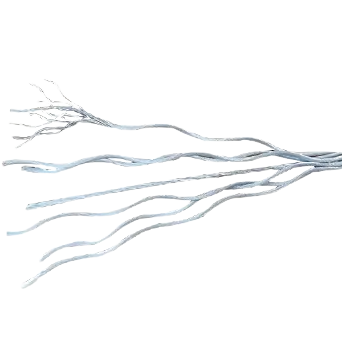
\includegraphics[scale=0.2]{rope-fiber.png}
\end{center}
    

\end{frame}

\begin{frame}{Fiber Cycle Breaking}{Issue with existing static scheduler}
    
Previously:
\begin{itemize}
    \item For every non-terminal whose fibered attributes take part in the cycle, created two \texttt{attribute\_decl} \alert{AST nodes} called up and down and the connected all nodes to these to break cycles and preserve only UP followed by DOWN.
\end{itemize}

Now:

\begin{itemize}
    \item \alert{No creation of AST node}. Treat all nodes as either up or down. If dependency is just fiber dependency then UP followed by DOWN. Otherwise, DOWN followed by UP.
\end{itemize}

\end{frame}


\begin{frame}{Fiber Cycle Breaking}{Validated!}

\alert{Drop-in replacement} algorithm was successful.

\begin{itemize}
    \item Validated the algorithm against \alert{previous APS codes} that contained only fiber cycles
    \item Validated the algorithm against \alert{First and Follow} APS codes 
\end{itemize}

\end{frame}


\begin{frame}{Static Scheduler}{Simplify scheduling by using groups}

Previously:
\begin{itemize}
    \item Naive \alert{greedy algorithm} that was hard to debug and \alert{tightly coupled with code generation} module
\end{itemize}
    
Now:
\begin{itemize}
    \item Scheduling using group is simpler, easier to debug and \alert{de-coupled from code generation} module.
    \item Includes $(\mathit{ph}, \mathit{ch})$ marker to help code generation identify the start and end of child visit.
\end{itemize}

\end{frame}


\begin{frame}{Static Scheduler}{Scheduling groups and $ph$ and $ch$ as group indicators}

The scheduler scheduled attribute in this order:
\begin{enumerate}
    \item A whole group of inherited attributes of the parent (start of a phase). This group could be empty $(-ph, -1)$
    \item A whole group of attributes (both inherited and synthesized) for a child phase  $(ph, ch)$
    \item A whole group of synthesized attributes of the parent (end the phase/visit). This group can be empty $(ph, -1)$
\end{enumerate}


 For the locals, it also makes sure they are scheduled according to the total order.
 
\end{frame}


\begin{frame}{Static Scheduler}{Validation in-progress ...}

\begin{itemize}
    \item Implementation is \alert{not finished yet}
\end{itemize}

\end{frame}